\documentclass[aspectratio=169]{beamer}

\usetheme{Madrid}
\usecolortheme{default}

\usepackage[utf8]{inputenc}
\usepackage[T1]{fontenc}
\usepackage{booktabs}
\usepackage{graphicx}
\usepackage{amsmath}

\graphicspath{{reports/figures/}}

\title[Electricity Load Forecasting Benchmark]{Benchmarking Machine Learning Models\\for Short-Term Electricity Load Forecasting}
\subtitle{Compact Data Science Benchmarking Prototype}
\author{Sharon Mathew PR}
\institute{M.Sc. Computational and Applied Mathematics, FAU}
\date{Working Student Data Scientist Interview}

\setbeamertemplate{navigation symbols}{}
\setbeamertemplate{footline}[frame number]

\begin{document}

\begin{frame}
    \titlepage
\end{frame}

\begin{frame}{Objective}
    \textbf{Goal:} build a compact benchmarking prototype for next-hour electricity load forecasting in Germany.

    \vspace{0.4cm}
    \begin{itemize}
        \item Predict short-term electricity load using historical hourly demand data.
        \item Compare simple and machine-learning models transparently.
        \item Verify whether ML models improve over a naive operational baseline.
        \item Produce reproducible outputs: metrics, plots, and clean project structure.
    \end{itemize}

    \vspace{0.3cm}
    \textbf{Framing:} data pipeline $\rightarrow$ features $\rightarrow$ model benchmark $\rightarrow$ evaluation $\rightarrow$ visualization.
\end{frame}

\begin{frame}{Data Used}
    \textbf{Source:} Open Power System Data, time series dataset.

    \vspace{0.3cm}
    \begin{itemize}
        \item File: \texttt{time\_series\_60min\_singleindex.csv}
        \item Frequency: hourly
        \item Raw file size: about 130 MB
        \item Raw rows: 50,401
        \item Timestamp: \texttt{utc\_timestamp}
        \item Target column: \texttt{DE\_load\_actual\_entsoe\_transparency}
    \end{itemize}

    \vspace{0.3cm}
    The target is renamed internally to \texttt{load\_mw}.

    \vspace{0.2cm}
    \textbf{Why UTC?} It avoids daylight-saving-time issues such as missing or repeated local hours.
\end{frame}

\begin{frame}{Preprocessing Pipeline}
    \begin{itemize}
        \item Read only required columns using \texttt{pandas.read\_csv(usecols=...)}.
        \item Parse timestamps and convert load values to numeric.
        \item Sort observations chronologically.
        \item Remove duplicate timestamps.
        \item Enforce hourly frequency.
        \item Interpolate only small internal gaps.
        \item Drop remaining missing load values.
    \end{itemize}

    \vspace{0.4cm}
    \textbf{Reasoning:} keep the pipeline robust, memory-efficient, and auditable before modeling.
\end{frame}

\begin{frame}{Feature Engineering}
    \textbf{Forecasting target:}
    \[
        target\_load\_mw_t = load\_mw_{t+1}
    \]

    \vspace{0.2cm}
    \begin{itemize}
        \item Calendar features: hour, day of week, month, weekend flag.
        \item Lag features: 1 hour, 24 hours, and 168 hours.
        \item Rolling features: 24-hour and 168-hour rolling mean and standard deviation.
    \end{itemize}

    \vspace{0.4cm}
    \textbf{Leakage prevention:}
    all lag and rolling features use only information available at or before the prediction origin.
\end{frame}

\begin{frame}{Validation Strategy}
    \textbf{Chronological train/test split}

    \vspace{0.3cm}
    \begin{itemize}
        \item First 80\% of prepared rows: training set.
        \item Final 20\% of prepared rows: test set.
        \item No shuffling, because forecasting must be evaluated on future unseen data.
        \item Final supervised modeling rows: 50,232.
    \end{itemize}

    \vspace{0.4cm}
    \textbf{Why this matters:} random splitting can leak future information and make performance look too optimistic.
\end{frame}

\begin{frame}{Models Benchmarked}
    \begin{table}
        \centering
        \begin{tabular}{p{0.28\linewidth} p{0.58\linewidth}}
            \toprule
            \textbf{Model} & \textbf{Motivation} \\
            \midrule
            Naive 24h Baseline & Same hour yesterday; simple operational benchmark. \\
            Ridge Regression & Regularized linear baseline; stable and explainable. \\
            Random Forest & Captures nonlinear relationships and feature interactions. \\
            HistGradientBoosting & Strong tabular model; sequentially corrects previous errors. \\
            \bottomrule
        \end{tabular}
    \end{table}

    \vspace{0.2cm}
    \textbf{Why these models fit:} electricity load has strong autocorrelation, daily seasonality, weekly seasonality, and nonlinear calendar effects.
\end{frame}

\begin{frame}{Evaluation Metrics}
    \begin{itemize}
        \item \textbf{MAE:} average absolute forecast error in MW.
        \item \textbf{RMSE:} penalizes larger errors more strongly.
        \item \textbf{MAPE:} average percentage error, with safe zero handling.
        \item \textbf{$R^2$:} variance explanation, used as a secondary metric.
    \end{itemize}

    \vspace{0.4cm}
    \textbf{Primary metric: MAE}

    \vspace{0.15cm}
    MAE is easy to explain to stakeholders because it stays in the original unit: megawatts.
\end{frame}

\begin{frame}{Benchmark Results}
    \begin{table}
        \centering
        \begin{tabular}{lrrrr}
            \toprule
            \textbf{Model} & \textbf{MAE} & \textbf{RMSE} & \textbf{MAPE} & \textbf{$R^2$} \\
            \midrule
            HistGradientBoosting & 537.05 & 719.03 & 1.03\% & 0.995 \\
            Random Forest & 559.28 & 765.19 & 1.07\% & 0.994 \\
            Ridge Regression & 1,282.24 & 1,695.95 & 2.48\% & 0.970 \\
            Naive 24h Baseline & 4,137.31 & 6,319.26 & 7.83\% & 0.588 \\
            \bottomrule
        \end{tabular}
    \end{table}

    \vspace{0.25cm}
    \textbf{Key finding:} HistGradientBoosting performed best and clearly improved over the naive baseline.
\end{frame}

\begin{frame}{Model Comparison Visualization}
    \centering
    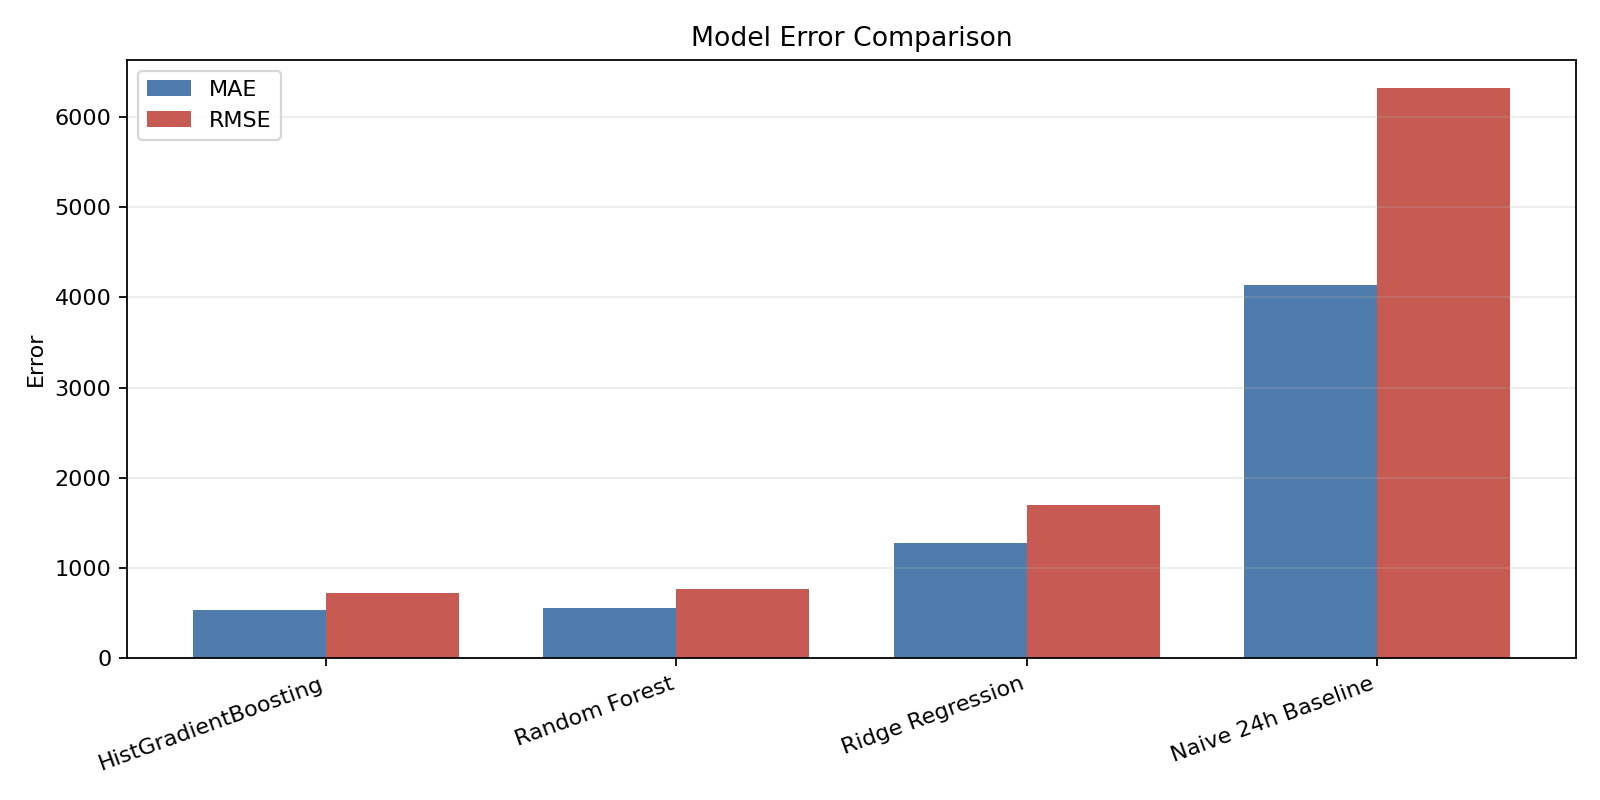
\includegraphics[width=0.88\linewidth]{05_model_metric_comparison.png}
\end{frame}

\begin{frame}{Actual vs Predicted: Final 14 Days}
    \centering
    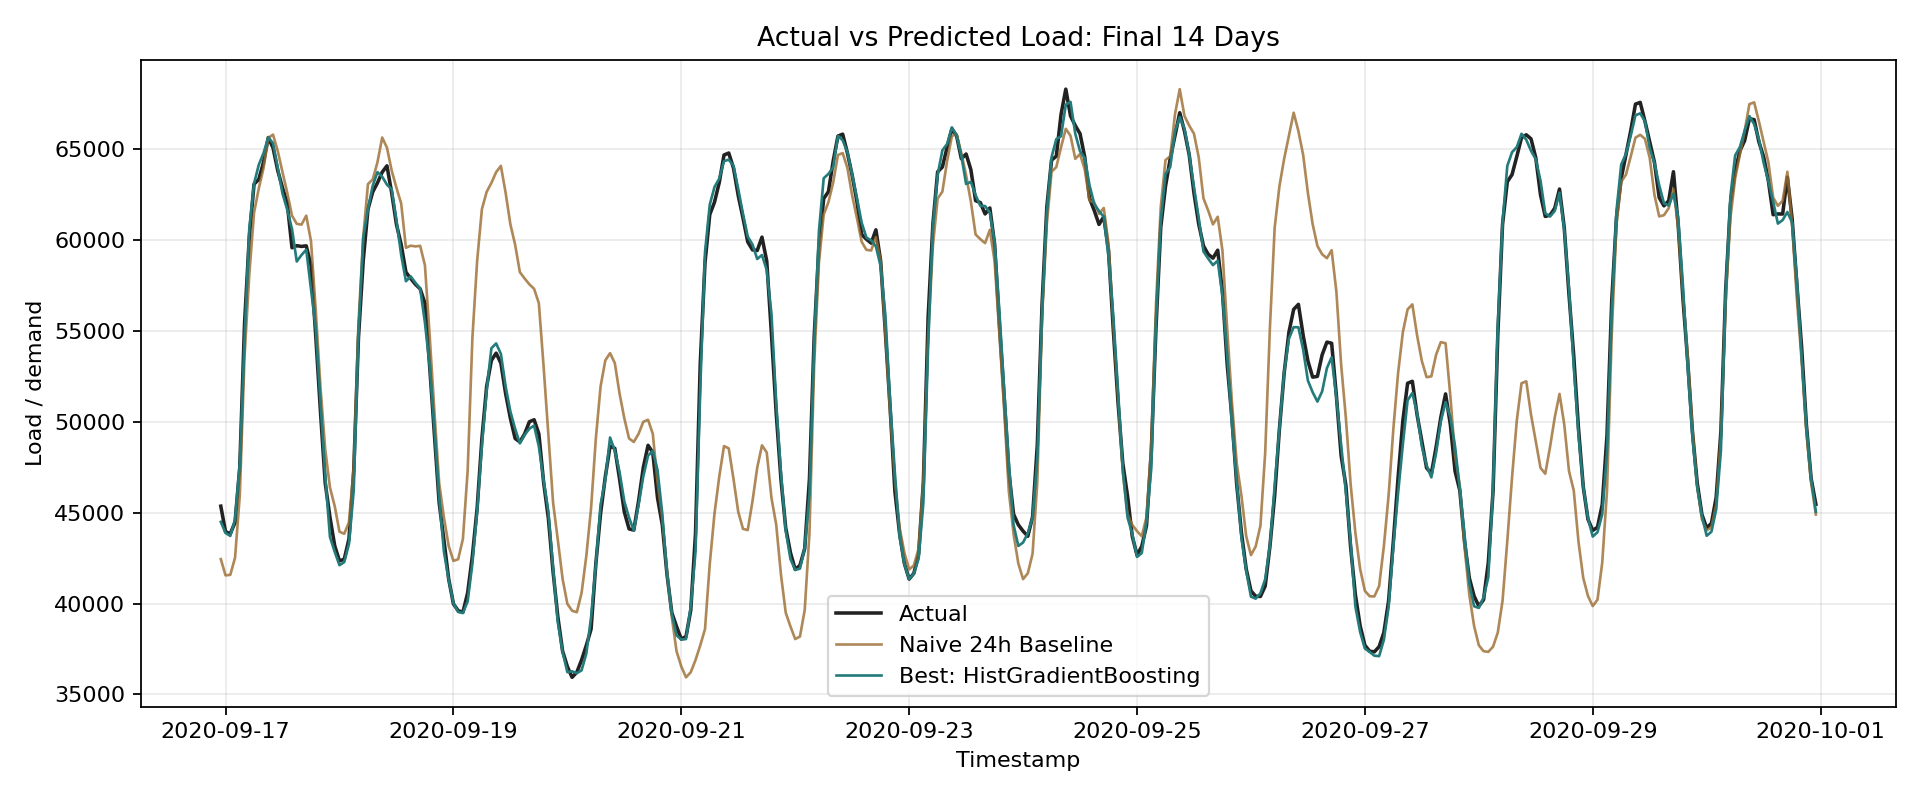
\includegraphics[width=0.92\linewidth]{04_actual_vs_predicted_final_14_days.png}

    \vspace{0.15cm}
    The best model tracks the daily load pattern much more closely than the naive baseline.
\end{frame}

\begin{frame}{Production-Minded Design}
    \begin{itemize}
        \item Modular code: data loading, preprocessing, features, models, evaluation, visualization.
        \item Cached raw data to avoid repeated large downloads.
        \item Chronological validation to avoid future leakage.
        \item Clear saved outputs for review and communication.
        \item Uses logging and configuration constants for reproducibility.
    \end{itemize}

    \vspace{0.35cm}
    \textbf{Interview message:} this is a small internal benchmarking prototype, not just a one-off notebook.
\end{frame}

\begin{frame}{Limitations and Next Steps}
    \textbf{Limitations}
    \begin{itemize}
        \item Uses only historical load and calendar features.
        \item Evaluates one chronological split, not full backtesting.
        \item Does not include weather, holidays, or external market signals.
    \end{itemize}

    \vspace{0.25cm}
    \textbf{Next steps}
    \begin{itemize}
        \item Add rolling or expanding-window backtesting.
        \item Evaluate stability by season, weekday/weekend, and peak periods.
        \item Add weather and holiday features.
        \item Add experiment tracking, model serialization, and a small prediction API.
    \end{itemize}
\end{frame}

\begin{frame}{Closing}
    \Large
    \textbf{Main takeaway}

    \vspace{0.4cm}
    \normalsize
    The project shows a clean workflow for benchmarking ML models on an operational forecasting problem:

    \vspace{0.25cm}
    \centering
    \textbf{high-quality data pipeline + leakage-safe validation + transparent model comparison}

    \vspace{0.45cm}
    \raggedright
    This matches the working-student data science role because it combines prototype building, model verification, visualization, and production-minded software structure.
\end{frame}

\end{document}
